\batchmode
\documentclass[twoside]{book}

% Packages required by doxygen
\usepackage{fixltx2e}
\usepackage{calc}
\usepackage{doxygen}
\usepackage[export]{adjustbox} % also loads graphicx
\usepackage{graphicx}
\usepackage[utf8]{inputenc}
\usepackage{makeidx}
\usepackage{multicol}
\usepackage{multirow}
\PassOptionsToPackage{warn}{textcomp}
\usepackage{textcomp}
\usepackage[nointegrals]{wasysym}
\usepackage[table]{xcolor}

% Font selection
\usepackage[T1]{fontenc}
\usepackage[scaled=.90]{helvet}
\usepackage{courier}
\usepackage{amssymb}
\usepackage{sectsty}
\renewcommand{\familydefault}{\sfdefault}
\allsectionsfont{%
  \fontseries{bc}\selectfont%
  \color{darkgray}%
}
\renewcommand{\DoxyLabelFont}{%
  \fontseries{bc}\selectfont%
  \color{darkgray}%
}
\newcommand{\+}{\discretionary{\mbox{\scriptsize$\hookleftarrow$}}{}{}}

% Page & text layout
\usepackage{geometry}
\geometry{%
  a4paper,%
  top=2.5cm,%
  bottom=2.5cm,%
  left=2.5cm,%
  right=2.5cm%
}
\tolerance=750
\hfuzz=15pt
\hbadness=750
\setlength{\emergencystretch}{15pt}
\setlength{\parindent}{0cm}
\setlength{\parskip}{3ex plus 2ex minus 2ex}
\makeatletter
\renewcommand{\paragraph}{%
  \@startsection{paragraph}{4}{0ex}{-1.0ex}{1.0ex}{%
    \normalfont\normalsize\bfseries\SS@parafont%
  }%
}
\renewcommand{\subparagraph}{%
  \@startsection{subparagraph}{5}{0ex}{-1.0ex}{1.0ex}{%
    \normalfont\normalsize\bfseries\SS@subparafont%
  }%
}
\makeatother

% Headers & footers
\usepackage{fancyhdr}
\pagestyle{fancyplain}
\fancyhead[LE]{\fancyplain{}{\bfseries\thepage}}
\fancyhead[CE]{\fancyplain{}{}}
\fancyhead[RE]{\fancyplain{}{\bfseries\leftmark}}
\fancyhead[LO]{\fancyplain{}{\bfseries\rightmark}}
\fancyhead[CO]{\fancyplain{}{}}
\fancyhead[RO]{\fancyplain{}{\bfseries\thepage}}
\fancyfoot[LE]{\fancyplain{}{}}
\fancyfoot[CE]{\fancyplain{}{}}
\fancyfoot[RE]{\fancyplain{}{\bfseries\scriptsize Generated by Doxygen }}
\fancyfoot[LO]{\fancyplain{}{\bfseries\scriptsize Generated by Doxygen }}
\fancyfoot[CO]{\fancyplain{}{}}
\fancyfoot[RO]{\fancyplain{}{}}
\renewcommand{\footrulewidth}{0.4pt}
\renewcommand{\chaptermark}[1]{%
  \markboth{#1}{}%
}
\renewcommand{\sectionmark}[1]{%
  \markright{\thesection\ #1}%
}

% Indices & bibliography
\usepackage{natbib}
\usepackage[titles]{tocloft}
\setcounter{tocdepth}{3}
\setcounter{secnumdepth}{5}
\makeindex

% Hyperlinks (required, but should be loaded last)
\usepackage{ifpdf}
\ifpdf
  \usepackage[pdftex,pagebackref=true]{hyperref}
\else
  \usepackage[ps2pdf,pagebackref=true]{hyperref}
\fi
\hypersetup{%
  colorlinks=true,%
  linkcolor=blue,%
  citecolor=blue,%
  unicode%
}

% Custom commands
\newcommand{\clearemptydoublepage}{%
  \newpage{\pagestyle{empty}\cleardoublepage}%
}

\usepackage{caption}
\captionsetup{labelsep=space,justification=centering,font={bf},singlelinecheck=off,skip=4pt,position=top}

%===== C O N T E N T S =====

\begin{document}

% Titlepage & ToC
\hypersetup{pageanchor=false,
             bookmarksnumbered=true
            }
\pagenumbering{alph}
\pagenumbering{arabic}
\hypersetup{pageanchor=true}

%--- Begin generated contents ---
\chapter{Example problem\+: S\+U\+P\+G-\/stabilised solution of the 2D advection diffusion equation}
\label{index}\hypertarget{index}{}\hypertarget{index_q}{}\section{A few quick questions...}\label{index_q}
Since {\ttfamily oomph-\/lib} is developed as open-\/source software, any evidence that the code is being downloaded and used is very helpful for us as it helps to justify our continued work on this project.

We would therefore be extremely grateful if you could provide the information requested in the form below. Pressing the \char`\"{}submit\char`\"{} button will get you to the actual download page.

{\bfseries Note\+:} 
\begin{DoxyItemize}
\item All information will be treated as confidential. 
\item If you provide your email address and check the appropriate box we will add you to our mailing list to inform you of upgrades and bug fixes to the code. Rest assured that the mailing list is {\bfseries very low volume} -- we have better things to do than to bombard you with email. 
\item If you still feel reluctant to provide any of the information requested, feel free to enter some dummy input. The form will check that {\bfseries some} information has been entered but entering your name as \char`\"{}\+Joe Cool\char`\"{} is perfectly acceptable -- this is to discourage people from not providing the information simply because they are too lazy to type... 
\end{DoxyItemize}



 







 

 \hypertarget{index_pdf}{}\section{P\+D\+F file}\label{index_pdf}
A \href{../latex/refman.pdf}{\tt pdf version} of this document is available. \end{document}

\chapter{Namespace Index}
\section{Namespace List}
Here is a list of all namespaces with brief descriptions\+:\begin{DoxyCompactList}
\item\contentsline{section}{\hyperlink{namespaceGlobal__Physical__Variables}{Global\+\_\+\+Physical\+\_\+\+Variables} \\*Global variables that represent physical properties }{\pageref{namespaceGlobal__Physical__Variables}}{}
\item\contentsline{section}{\hyperlink{namespaceoomph}{oomph} }{\pageref{namespaceoomph}}{}
\item\contentsline{section}{\hyperlink{namespacePhysical__Variables}{Physical\+\_\+\+Variables} \\*Namespace for the solution of 2D linear shell equation }{\pageref{namespacePhysical__Variables}}{}
\end{DoxyCompactList}

\chapter{Hierarchical Index}
\section{Class Hierarchy}
This inheritance list is sorted roughly, but not completely, alphabetically\+:\begin{DoxyCompactList}
\item Problem\begin{DoxyCompactList}
\item \contentsline{section}{Unstructured\+Solid\+Problem$<$ E\+L\+E\+M\+E\+NT $>$}{\pageref{classUnstructuredSolidProblem}}{}
\end{DoxyCompactList}
\end{DoxyCompactList}

\chapter{Class Index}
\section{Class List}
Here are the classes, structs, unions and interfaces with brief descriptions\+:\begin{DoxyCompactList}
\item\contentsline{section}{\hyperlink{classPMLProblem}{P\+M\+L\+Problem$<$ E\+L\+E\+M\+E\+N\+T $>$} }{\pageref{classPMLProblem}}{}
\item\contentsline{section}{\hyperlink{classGlobalParameters_1_1TestPMLMapping}{Global\+Parameters\+::\+Test\+P\+M\+L\+Mapping} }{\pageref{classGlobalParameters_1_1TestPMLMapping}}{}
\end{DoxyCompactList}

\chapter{File Index}
\section{File List}
Here is a list of all files with brief descriptions\+:\begin{DoxyCompactList}
\item\contentsline{section}{\hyperlink{jeffery__orbit_8cc}{jeffery\+\_\+orbit.\+cc} }{\pageref{jeffery__orbit_8cc}}{}
\item\contentsline{section}{\hyperlink{jeffery__orbit_8txt__doxygenified_8h}{jeffery\+\_\+orbit.\+txt\+\_\+doxygenified.\+h} }{\pageref{jeffery__orbit_8txt__doxygenified_8h}}{}
\item\contentsline{section}{\hyperlink{my__taylor__hood__elements_8h}{my\+\_\+taylor\+\_\+hood\+\_\+elements.\+h} }{\pageref{my__taylor__hood__elements_8h}}{}
\end{DoxyCompactList}

\chapter{Namespace Documentation}
\hypertarget{namespaceGlobalPhysicalParameters}{}\section{Global\+Physical\+Parameters Namespace Reference}
\label{namespaceGlobalPhysicalParameters}\index{Global\+Physical\+Parameters@{Global\+Physical\+Parameters}}
\subsection*{Functions}
\begin{DoxyCompactItemize}
\item 
void \hyperlink{namespaceGlobalPhysicalParameters_a6e1db5726436a705e9d400fedf914cef}{get\+\_\+boundary\+\_\+values} (const Vector$<$ double $>$ \&x, Vector$<$ double $>$ \&u)
\begin{DoxyCompactList}\small\item\em Some \char`\"{}solution\char`\"{} for assignment of boundary values. \end{DoxyCompactList}\item 
void \hyperlink{namespaceGlobalPhysicalParameters_aa84986d4d50cb043cc8fced56feab45f}{source\+\_\+function} (const Vector$<$ double $>$ \&x\+\_\+vect, double \&source)
\begin{DoxyCompactList}\small\item\em Zero source function. \end{DoxyCompactList}\item 
void \hyperlink{namespaceGlobalPhysicalParameters_a3a17e62bc0096244627f5f1a7f53c859}{wind\+\_\+function} (const Vector$<$ double $>$ \&x, Vector$<$ double $>$ \&wind)
\begin{DoxyCompactList}\small\item\em Wind. \end{DoxyCompactList}\end{DoxyCompactItemize}
\subsection*{Variables}
\begin{DoxyCompactItemize}
\item 
double \hyperlink{namespaceGlobalPhysicalParameters_ab7011a8f93f2cbd3d45af00151aee3b2}{Peclet} =200.\+0
\begin{DoxyCompactList}\small\item\em Peclet number. \end{DoxyCompactList}\item 
double \hyperlink{namespaceGlobalPhysicalParameters_aec7a344b74b10d835b331ef0dc6601da}{Alpha} =50.\+0
\begin{DoxyCompactList}\small\item\em Parameter for steepness of step in boundary values. \end{DoxyCompactList}\item 
double \hyperlink{namespaceGlobalPhysicalParameters_af9a5a947d725f1f088db6a6423f2f3ef}{Tan\+Phi} =1.\+0
\begin{DoxyCompactList}\small\item\em Parameter for angle of step in boundary values\+: 45 degrees. \end{DoxyCompactList}\end{DoxyCompactItemize}


\subsection{Detailed Description}
Namespace for global parameters\+: Unforced problem with boundary values corresponding to a steep tanh step profile oriented at 45 degrees across the domain. 

\subsection{Function Documentation}
\mbox{\Hypertarget{namespaceGlobalPhysicalParameters_a6e1db5726436a705e9d400fedf914cef}\label{namespaceGlobalPhysicalParameters_a6e1db5726436a705e9d400fedf914cef}} 
\index{Global\+Physical\+Parameters@{Global\+Physical\+Parameters}!get\+\_\+boundary\+\_\+values@{get\+\_\+boundary\+\_\+values}}
\index{get\+\_\+boundary\+\_\+values@{get\+\_\+boundary\+\_\+values}!Global\+Physical\+Parameters@{Global\+Physical\+Parameters}}
\subsubsection{\texorpdfstring{get\+\_\+boundary\+\_\+values()}{get\_boundary\_values()}}
{\footnotesize\ttfamily void Global\+Physical\+Parameters\+::get\+\_\+boundary\+\_\+values (\begin{DoxyParamCaption}\item[{const Vector$<$ double $>$ \&}]{x,  }\item[{Vector$<$ double $>$ \&}]{u }\end{DoxyParamCaption})}



Some \char`\"{}solution\char`\"{} for assignment of boundary values. 



Definition at line 65 of file two\+\_\+d\+\_\+adv\+\_\+diff\+\_\+\+S\+U\+P\+G.\+cc.



Referenced by S\+U\+P\+G\+Advection\+Diffusion\+Problem$<$ E\+L\+E\+M\+E\+N\+T $>$\+::actions\+\_\+before\+\_\+newton\+\_\+solve().

\mbox{\Hypertarget{namespaceGlobalPhysicalParameters_aa84986d4d50cb043cc8fced56feab45f}\label{namespaceGlobalPhysicalParameters_aa84986d4d50cb043cc8fced56feab45f}} 
\index{Global\+Physical\+Parameters@{Global\+Physical\+Parameters}!source\+\_\+function@{source\+\_\+function}}
\index{source\+\_\+function@{source\+\_\+function}!Global\+Physical\+Parameters@{Global\+Physical\+Parameters}}
\subsubsection{\texorpdfstring{source\+\_\+function()}{source\_function()}}
{\footnotesize\ttfamily void Global\+Physical\+Parameters\+::source\+\_\+function (\begin{DoxyParamCaption}\item[{const Vector$<$ double $>$ \&}]{x\+\_\+vect,  }\item[{double \&}]{source }\end{DoxyParamCaption})}



Zero source function. 



Definition at line 71 of file two\+\_\+d\+\_\+adv\+\_\+diff\+\_\+\+S\+U\+P\+G.\+cc.



Referenced by main().

\mbox{\Hypertarget{namespaceGlobalPhysicalParameters_a3a17e62bc0096244627f5f1a7f53c859}\label{namespaceGlobalPhysicalParameters_a3a17e62bc0096244627f5f1a7f53c859}} 
\index{Global\+Physical\+Parameters@{Global\+Physical\+Parameters}!wind\+\_\+function@{wind\+\_\+function}}
\index{wind\+\_\+function@{wind\+\_\+function}!Global\+Physical\+Parameters@{Global\+Physical\+Parameters}}
\subsubsection{\texorpdfstring{wind\+\_\+function()}{wind\_function()}}
{\footnotesize\ttfamily void Global\+Physical\+Parameters\+::wind\+\_\+function (\begin{DoxyParamCaption}\item[{const Vector$<$ double $>$ \&}]{x,  }\item[{Vector$<$ double $>$ \&}]{wind }\end{DoxyParamCaption})}



Wind. 



Definition at line 77 of file two\+\_\+d\+\_\+adv\+\_\+diff\+\_\+\+S\+U\+P\+G.\+cc.



Referenced by main().



\subsection{Variable Documentation}
\mbox{\Hypertarget{namespaceGlobalPhysicalParameters_aec7a344b74b10d835b331ef0dc6601da}\label{namespaceGlobalPhysicalParameters_aec7a344b74b10d835b331ef0dc6601da}} 
\index{Global\+Physical\+Parameters@{Global\+Physical\+Parameters}!Alpha@{Alpha}}
\index{Alpha@{Alpha}!Global\+Physical\+Parameters@{Global\+Physical\+Parameters}}
\subsubsection{\texorpdfstring{Alpha}{Alpha}}
{\footnotesize\ttfamily double Global\+Physical\+Parameters\+::\+Alpha =50.\+0}



Parameter for steepness of step in boundary values. 



Definition at line 59 of file two\+\_\+d\+\_\+adv\+\_\+diff\+\_\+\+S\+U\+P\+G.\+cc.

\mbox{\Hypertarget{namespaceGlobalPhysicalParameters_ab7011a8f93f2cbd3d45af00151aee3b2}\label{namespaceGlobalPhysicalParameters_ab7011a8f93f2cbd3d45af00151aee3b2}} 
\index{Global\+Physical\+Parameters@{Global\+Physical\+Parameters}!Peclet@{Peclet}}
\index{Peclet@{Peclet}!Global\+Physical\+Parameters@{Global\+Physical\+Parameters}}
\subsubsection{\texorpdfstring{Peclet}{Peclet}}
{\footnotesize\ttfamily double Global\+Physical\+Parameters\+::\+Peclet =200.\+0}



Peclet number. 



Definition at line 56 of file two\+\_\+d\+\_\+adv\+\_\+diff\+\_\+\+S\+U\+P\+G.\+cc.



Referenced by S\+U\+P\+G\+Advection\+Diffusion\+Problem$<$ E\+L\+E\+M\+E\+N\+T $>$\+::\+S\+U\+P\+G\+Advection\+Diffusion\+Problem().

\mbox{\Hypertarget{namespaceGlobalPhysicalParameters_af9a5a947d725f1f088db6a6423f2f3ef}\label{namespaceGlobalPhysicalParameters_af9a5a947d725f1f088db6a6423f2f3ef}} 
\index{Global\+Physical\+Parameters@{Global\+Physical\+Parameters}!Tan\+Phi@{Tan\+Phi}}
\index{Tan\+Phi@{Tan\+Phi}!Global\+Physical\+Parameters@{Global\+Physical\+Parameters}}
\subsubsection{\texorpdfstring{Tan\+Phi}{TanPhi}}
{\footnotesize\ttfamily double Global\+Physical\+Parameters\+::\+Tan\+Phi =1.\+0}



Parameter for angle of step in boundary values\+: 45 degrees. 



Definition at line 62 of file two\+\_\+d\+\_\+adv\+\_\+diff\+\_\+\+S\+U\+P\+G.\+cc.


\chapter{Class Documentation}
\hypertarget{classSUPGAdvectionDiffusionProblem}{}\section{S\+U\+P\+G\+Advection\+Diffusion\+Problem$<$ E\+L\+E\+M\+E\+NT $>$ Class Template Reference}
\label{classSUPGAdvectionDiffusionProblem}\index{S\+U\+P\+G\+Advection\+Diffusion\+Problem$<$ E\+L\+E\+M\+E\+N\+T $>$@{S\+U\+P\+G\+Advection\+Diffusion\+Problem$<$ E\+L\+E\+M\+E\+N\+T $>$}}
Inheritance diagram for S\+U\+P\+G\+Advection\+Diffusion\+Problem$<$ E\+L\+E\+M\+E\+NT $>$\+:\begin{figure}[H]
\begin{center}
\leavevmode
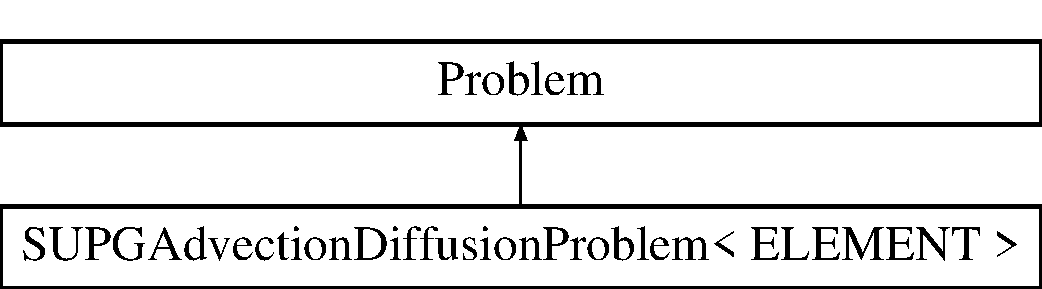
\includegraphics[height=2.000000cm]{classSUPGAdvectionDiffusionProblem}
\end{center}
\end{figure}
\subsection*{Public Member Functions}
\begin{DoxyCompactItemize}
\item 
\hyperlink{classSUPGAdvectionDiffusionProblem_a95aa4192c1b42327b12cdbb75295d192}{S\+U\+P\+G\+Advection\+Diffusion\+Problem} (Advection\+Diffusion\+Equations$<$ 2 $>$\+::Advection\+Diffusion\+Source\+Fct\+Pt source\+\_\+fct\+\_\+pt, Advection\+Diffusion\+Equations$<$ 2 $>$\+::Advection\+Diffusion\+Wind\+Fct\+Pt wind\+\_\+fct\+\_\+pt, const bool \&use\+\_\+stabilisation)
\begin{DoxyCompactList}\small\item\em Constructor\+: Pass pointer to source and wind functions, and flag to indicate if stabilisation is to be used. \end{DoxyCompactList}\item 
\hyperlink{classSUPGAdvectionDiffusionProblem_a2112492d8a8a2ad9c0d8ef79e892ebd1}{$\sim$\+S\+U\+P\+G\+Advection\+Diffusion\+Problem} ()
\begin{DoxyCompactList}\small\item\em Destructor. Empty. \end{DoxyCompactList}\item 
void \hyperlink{classSUPGAdvectionDiffusionProblem_affa45863033de517e1fba088aaae7eb5}{actions\+\_\+before\+\_\+newton\+\_\+solve} ()
\begin{DoxyCompactList}\small\item\em Update the problem specs before solve\+: Reset boundary conditions to the values from the tanh solution and compute stabilisation parameter. \end{DoxyCompactList}\item 
void \hyperlink{classSUPGAdvectionDiffusionProblem_a7ca10f3d82af3c3fec4c1a3260062ff2}{actions\+\_\+after\+\_\+newton\+\_\+solve} ()
\begin{DoxyCompactList}\small\item\em Update the problem after solve (empty) \end{DoxyCompactList}\item 
void \hyperlink{classSUPGAdvectionDiffusionProblem_a3133ba26f0917f5d210d69ea0ddcb1fe}{doc\+\_\+solution} ()
\begin{DoxyCompactList}\small\item\em Doc the solution. \end{DoxyCompactList}\item 
Rectangular\+Quad\+Mesh$<$ E\+L\+E\+M\+E\+NT $>$ $\ast$ \hyperlink{classSUPGAdvectionDiffusionProblem_ac54d5c05b91ca542e66760b2f1dd67c9}{mesh\+\_\+pt} ()
\begin{DoxyCompactList}\small\item\em Overloaded version of the problem\textquotesingle{}s access function to the mesh. Recasts the pointer to the base Mesh object to the actual mesh type. \end{DoxyCompactList}\end{DoxyCompactItemize}
\subsection*{Private Attributes}
\begin{DoxyCompactItemize}
\item 
Doc\+Info \hyperlink{classSUPGAdvectionDiffusionProblem_af80606875e03033c0de217f7a861d0af}{Doc\+\_\+info}
\begin{DoxyCompactList}\small\item\em Doc\+Info object. \end{DoxyCompactList}\item 
Advection\+Diffusion\+Equations$<$ 2 $>$\+::Advection\+Diffusion\+Source\+Fct\+Pt \hyperlink{classSUPGAdvectionDiffusionProblem_a9bf04de8641dd4151514c2e2603f3ac5}{Source\+\_\+fct\+\_\+pt}
\begin{DoxyCompactList}\small\item\em Pointer to source function. \end{DoxyCompactList}\item 
Advection\+Diffusion\+Equations$<$ 2 $>$\+::Advection\+Diffusion\+Wind\+Fct\+Pt \hyperlink{classSUPGAdvectionDiffusionProblem_a89bc22484946ccf51bb7cf7328bc9df6}{Wind\+\_\+fct\+\_\+pt}
\begin{DoxyCompactList}\small\item\em Pointer to wind function. \end{DoxyCompactList}\item 
bool \hyperlink{classSUPGAdvectionDiffusionProblem_ab8c19428c17ac7d8bb776e91940734bd}{Use\+\_\+stabilisation}
\begin{DoxyCompactList}\small\item\em Flag to indicate if stabilisation is to be used. \end{DoxyCompactList}\end{DoxyCompactItemize}


\subsection{Detailed Description}
\subsubsection*{template$<$class E\+L\+E\+M\+E\+NT$>$\newline
class S\+U\+P\+G\+Advection\+Diffusion\+Problem$<$ E\+L\+E\+M\+E\+N\+T $>$}

2D Advection\+Diffusion problem on rectangular domain, discretised with refineable 2D Q\+Advection\+Diffusion elements. The specific type of element is specified via the template parameter. 

Definition at line 97 of file two\+\_\+d\+\_\+adv\+\_\+diff\+\_\+\+S\+U\+P\+G.\+cc.



\subsection{Constructor \& Destructor Documentation}
\mbox{\Hypertarget{classSUPGAdvectionDiffusionProblem_a95aa4192c1b42327b12cdbb75295d192}\label{classSUPGAdvectionDiffusionProblem_a95aa4192c1b42327b12cdbb75295d192}} 
\index{S\+U\+P\+G\+Advection\+Diffusion\+Problem@{S\+U\+P\+G\+Advection\+Diffusion\+Problem}!S\+U\+P\+G\+Advection\+Diffusion\+Problem@{S\+U\+P\+G\+Advection\+Diffusion\+Problem}}
\index{S\+U\+P\+G\+Advection\+Diffusion\+Problem@{S\+U\+P\+G\+Advection\+Diffusion\+Problem}!S\+U\+P\+G\+Advection\+Diffusion\+Problem@{S\+U\+P\+G\+Advection\+Diffusion\+Problem}}
\subsubsection{\texorpdfstring{S\+U\+P\+G\+Advection\+Diffusion\+Problem()}{SUPGAdvectionDiffusionProblem()}}
{\footnotesize\ttfamily template$<$class E\+L\+E\+M\+E\+NT $>$ \\
\hyperlink{classSUPGAdvectionDiffusionProblem}{S\+U\+P\+G\+Advection\+Diffusion\+Problem}$<$ E\+L\+E\+M\+E\+NT $>$\+::\hyperlink{classSUPGAdvectionDiffusionProblem}{S\+U\+P\+G\+Advection\+Diffusion\+Problem} (\begin{DoxyParamCaption}\item[{Advection\+Diffusion\+Equations$<$ 2 $>$\+::Advection\+Diffusion\+Source\+Fct\+Pt}]{source\+\_\+fct\+\_\+pt,  }\item[{Advection\+Diffusion\+Equations$<$ 2 $>$\+::Advection\+Diffusion\+Wind\+Fct\+Pt}]{wind\+\_\+fct\+\_\+pt,  }\item[{const bool \&}]{use\+\_\+stabilisation }\end{DoxyParamCaption})}



Constructor\+: Pass pointer to source and wind functions, and flag to indicate if stabilisation is to be used. 

Constructor for Advection\+Diffusion problem\+: Pass pointer to source function and wind functions and flag to indicate if stabilisation is to be used. 

Definition at line 156 of file two\+\_\+d\+\_\+adv\+\_\+diff\+\_\+\+S\+U\+P\+G.\+cc.



References S\+U\+P\+G\+Advection\+Diffusion\+Problem$<$ E\+L\+E\+M\+E\+N\+T $>$\+::\+Doc\+\_\+info, S\+U\+P\+G\+Advection\+Diffusion\+Problem$<$ E\+L\+E\+M\+E\+N\+T $>$\+::mesh\+\_\+pt(), Global\+Physical\+Parameters\+::\+Peclet, S\+U\+P\+G\+Advection\+Diffusion\+Problem$<$ E\+L\+E\+M\+E\+N\+T $>$\+::\+Source\+\_\+fct\+\_\+pt, and S\+U\+P\+G\+Advection\+Diffusion\+Problem$<$ E\+L\+E\+M\+E\+N\+T $>$\+::\+Wind\+\_\+fct\+\_\+pt.

\mbox{\Hypertarget{classSUPGAdvectionDiffusionProblem_a2112492d8a8a2ad9c0d8ef79e892ebd1}\label{classSUPGAdvectionDiffusionProblem_a2112492d8a8a2ad9c0d8ef79e892ebd1}} 
\index{S\+U\+P\+G\+Advection\+Diffusion\+Problem@{S\+U\+P\+G\+Advection\+Diffusion\+Problem}!````~S\+U\+P\+G\+Advection\+Diffusion\+Problem@{$\sim$\+S\+U\+P\+G\+Advection\+Diffusion\+Problem}}
\index{````~S\+U\+P\+G\+Advection\+Diffusion\+Problem@{$\sim$\+S\+U\+P\+G\+Advection\+Diffusion\+Problem}!S\+U\+P\+G\+Advection\+Diffusion\+Problem@{S\+U\+P\+G\+Advection\+Diffusion\+Problem}}
\subsubsection{\texorpdfstring{$\sim$\+S\+U\+P\+G\+Advection\+Diffusion\+Problem()}{~SUPGAdvectionDiffusionProblem()}}
{\footnotesize\ttfamily template$<$class E\+L\+E\+M\+E\+NT$>$ \\
\hyperlink{classSUPGAdvectionDiffusionProblem}{S\+U\+P\+G\+Advection\+Diffusion\+Problem}$<$ E\+L\+E\+M\+E\+NT $>$\+::$\sim$\hyperlink{classSUPGAdvectionDiffusionProblem}{S\+U\+P\+G\+Advection\+Diffusion\+Problem} (\begin{DoxyParamCaption}{ }\end{DoxyParamCaption})\hspace{0.3cm}{\ttfamily [inline]}}



Destructor. Empty. 



Definition at line 110 of file two\+\_\+d\+\_\+adv\+\_\+diff\+\_\+\+S\+U\+P\+G.\+cc.



\subsection{Member Function Documentation}
\mbox{\Hypertarget{classSUPGAdvectionDiffusionProblem_a7ca10f3d82af3c3fec4c1a3260062ff2}\label{classSUPGAdvectionDiffusionProblem_a7ca10f3d82af3c3fec4c1a3260062ff2}} 
\index{S\+U\+P\+G\+Advection\+Diffusion\+Problem@{S\+U\+P\+G\+Advection\+Diffusion\+Problem}!actions\+\_\+after\+\_\+newton\+\_\+solve@{actions\+\_\+after\+\_\+newton\+\_\+solve}}
\index{actions\+\_\+after\+\_\+newton\+\_\+solve@{actions\+\_\+after\+\_\+newton\+\_\+solve}!S\+U\+P\+G\+Advection\+Diffusion\+Problem@{S\+U\+P\+G\+Advection\+Diffusion\+Problem}}
\subsubsection{\texorpdfstring{actions\+\_\+after\+\_\+newton\+\_\+solve()}{actions\_after\_newton\_solve()}}
{\footnotesize\ttfamily template$<$class E\+L\+E\+M\+E\+NT$>$ \\
void \hyperlink{classSUPGAdvectionDiffusionProblem}{S\+U\+P\+G\+Advection\+Diffusion\+Problem}$<$ E\+L\+E\+M\+E\+NT $>$\+::actions\+\_\+after\+\_\+newton\+\_\+solve (\begin{DoxyParamCaption}{ }\end{DoxyParamCaption})\hspace{0.3cm}{\ttfamily [inline]}}



Update the problem after solve (empty) 



Definition at line 118 of file two\+\_\+d\+\_\+adv\+\_\+diff\+\_\+\+S\+U\+P\+G.\+cc.

\mbox{\Hypertarget{classSUPGAdvectionDiffusionProblem_affa45863033de517e1fba088aaae7eb5}\label{classSUPGAdvectionDiffusionProblem_affa45863033de517e1fba088aaae7eb5}} 
\index{S\+U\+P\+G\+Advection\+Diffusion\+Problem@{S\+U\+P\+G\+Advection\+Diffusion\+Problem}!actions\+\_\+before\+\_\+newton\+\_\+solve@{actions\+\_\+before\+\_\+newton\+\_\+solve}}
\index{actions\+\_\+before\+\_\+newton\+\_\+solve@{actions\+\_\+before\+\_\+newton\+\_\+solve}!S\+U\+P\+G\+Advection\+Diffusion\+Problem@{S\+U\+P\+G\+Advection\+Diffusion\+Problem}}
\subsubsection{\texorpdfstring{actions\+\_\+before\+\_\+newton\+\_\+solve()}{actions\_before\_newton\_solve()}}
{\footnotesize\ttfamily template$<$class E\+L\+E\+M\+E\+NT $>$ \\
void \hyperlink{classSUPGAdvectionDiffusionProblem}{S\+U\+P\+G\+Advection\+Diffusion\+Problem}$<$ E\+L\+E\+M\+E\+NT $>$\+::actions\+\_\+before\+\_\+newton\+\_\+solve (\begin{DoxyParamCaption}{ }\end{DoxyParamCaption})}



Update the problem specs before solve\+: Reset boundary conditions to the values from the tanh solution and compute stabilisation parameter. 

Update the problem specs before solve\+: (Re-\/)set boundary conditions. 

Definition at line 237 of file two\+\_\+d\+\_\+adv\+\_\+diff\+\_\+\+S\+U\+P\+G.\+cc.



References Global\+Physical\+Parameters\+::get\+\_\+boundary\+\_\+values(), S\+U\+P\+G\+Advection\+Diffusion\+Problem$<$ E\+L\+E\+M\+E\+N\+T $>$\+::mesh\+\_\+pt(), and S\+U\+P\+G\+Advection\+Diffusion\+Problem$<$ E\+L\+E\+M\+E\+N\+T $>$\+::\+Use\+\_\+stabilisation.

\mbox{\Hypertarget{classSUPGAdvectionDiffusionProblem_a3133ba26f0917f5d210d69ea0ddcb1fe}\label{classSUPGAdvectionDiffusionProblem_a3133ba26f0917f5d210d69ea0ddcb1fe}} 
\index{S\+U\+P\+G\+Advection\+Diffusion\+Problem@{S\+U\+P\+G\+Advection\+Diffusion\+Problem}!doc\+\_\+solution@{doc\+\_\+solution}}
\index{doc\+\_\+solution@{doc\+\_\+solution}!S\+U\+P\+G\+Advection\+Diffusion\+Problem@{S\+U\+P\+G\+Advection\+Diffusion\+Problem}}
\subsubsection{\texorpdfstring{doc\+\_\+solution()}{doc\_solution()}}
{\footnotesize\ttfamily template$<$class E\+L\+E\+M\+E\+NT $>$ \\
void \hyperlink{classSUPGAdvectionDiffusionProblem}{S\+U\+P\+G\+Advection\+Diffusion\+Problem}$<$ E\+L\+E\+M\+E\+NT $>$\+::doc\+\_\+solution (\begin{DoxyParamCaption}{ }\end{DoxyParamCaption})}



Doc the solution. 



Definition at line 298 of file two\+\_\+d\+\_\+adv\+\_\+diff\+\_\+\+S\+U\+P\+G.\+cc.



References S\+U\+P\+G\+Advection\+Diffusion\+Problem$<$ E\+L\+E\+M\+E\+N\+T $>$\+::\+Doc\+\_\+info, and S\+U\+P\+G\+Advection\+Diffusion\+Problem$<$ E\+L\+E\+M\+E\+N\+T $>$\+::mesh\+\_\+pt().



Referenced by main().

\mbox{\Hypertarget{classSUPGAdvectionDiffusionProblem_ac54d5c05b91ca542e66760b2f1dd67c9}\label{classSUPGAdvectionDiffusionProblem_ac54d5c05b91ca542e66760b2f1dd67c9}} 
\index{S\+U\+P\+G\+Advection\+Diffusion\+Problem@{S\+U\+P\+G\+Advection\+Diffusion\+Problem}!mesh\+\_\+pt@{mesh\+\_\+pt}}
\index{mesh\+\_\+pt@{mesh\+\_\+pt}!S\+U\+P\+G\+Advection\+Diffusion\+Problem@{S\+U\+P\+G\+Advection\+Diffusion\+Problem}}
\subsubsection{\texorpdfstring{mesh\+\_\+pt()}{mesh\_pt()}}
{\footnotesize\ttfamily template$<$class E\+L\+E\+M\+E\+NT$>$ \\
Rectangular\+Quad\+Mesh$<$E\+L\+E\+M\+E\+NT$>$$\ast$ \hyperlink{classSUPGAdvectionDiffusionProblem}{S\+U\+P\+G\+Advection\+Diffusion\+Problem}$<$ E\+L\+E\+M\+E\+NT $>$\+::mesh\+\_\+pt (\begin{DoxyParamCaption}{ }\end{DoxyParamCaption})\hspace{0.3cm}{\ttfamily [inline]}}



Overloaded version of the problem\textquotesingle{}s access function to the mesh. Recasts the pointer to the base Mesh object to the actual mesh type. 



Definition at line 126 of file two\+\_\+d\+\_\+adv\+\_\+diff\+\_\+\+S\+U\+P\+G.\+cc.



Referenced by S\+U\+P\+G\+Advection\+Diffusion\+Problem$<$ E\+L\+E\+M\+E\+N\+T $>$\+::actions\+\_\+before\+\_\+newton\+\_\+solve(), S\+U\+P\+G\+Advection\+Diffusion\+Problem$<$ E\+L\+E\+M\+E\+N\+T $>$\+::doc\+\_\+solution(), and S\+U\+P\+G\+Advection\+Diffusion\+Problem$<$ E\+L\+E\+M\+E\+N\+T $>$\+::\+S\+U\+P\+G\+Advection\+Diffusion\+Problem().



\subsection{Member Data Documentation}
\mbox{\Hypertarget{classSUPGAdvectionDiffusionProblem_af80606875e03033c0de217f7a861d0af}\label{classSUPGAdvectionDiffusionProblem_af80606875e03033c0de217f7a861d0af}} 
\index{S\+U\+P\+G\+Advection\+Diffusion\+Problem@{S\+U\+P\+G\+Advection\+Diffusion\+Problem}!Doc\+\_\+info@{Doc\+\_\+info}}
\index{Doc\+\_\+info@{Doc\+\_\+info}!S\+U\+P\+G\+Advection\+Diffusion\+Problem@{S\+U\+P\+G\+Advection\+Diffusion\+Problem}}
\subsubsection{\texorpdfstring{Doc\+\_\+info}{Doc\_info}}
{\footnotesize\ttfamily template$<$class E\+L\+E\+M\+E\+NT$>$ \\
Doc\+Info \hyperlink{classSUPGAdvectionDiffusionProblem}{S\+U\+P\+G\+Advection\+Diffusion\+Problem}$<$ E\+L\+E\+M\+E\+NT $>$\+::Doc\+\_\+info\hspace{0.3cm}{\ttfamily [private]}}



Doc\+Info object. 



Definition at line 135 of file two\+\_\+d\+\_\+adv\+\_\+diff\+\_\+\+S\+U\+P\+G.\+cc.



Referenced by S\+U\+P\+G\+Advection\+Diffusion\+Problem$<$ E\+L\+E\+M\+E\+N\+T $>$\+::doc\+\_\+solution(), and S\+U\+P\+G\+Advection\+Diffusion\+Problem$<$ E\+L\+E\+M\+E\+N\+T $>$\+::\+S\+U\+P\+G\+Advection\+Diffusion\+Problem().

\mbox{\Hypertarget{classSUPGAdvectionDiffusionProblem_a9bf04de8641dd4151514c2e2603f3ac5}\label{classSUPGAdvectionDiffusionProblem_a9bf04de8641dd4151514c2e2603f3ac5}} 
\index{S\+U\+P\+G\+Advection\+Diffusion\+Problem@{S\+U\+P\+G\+Advection\+Diffusion\+Problem}!Source\+\_\+fct\+\_\+pt@{Source\+\_\+fct\+\_\+pt}}
\index{Source\+\_\+fct\+\_\+pt@{Source\+\_\+fct\+\_\+pt}!S\+U\+P\+G\+Advection\+Diffusion\+Problem@{S\+U\+P\+G\+Advection\+Diffusion\+Problem}}
\subsubsection{\texorpdfstring{Source\+\_\+fct\+\_\+pt}{Source\_fct\_pt}}
{\footnotesize\ttfamily template$<$class E\+L\+E\+M\+E\+NT$>$ \\
Advection\+Diffusion\+Equations$<$2$>$\+::Advection\+Diffusion\+Source\+Fct\+Pt \hyperlink{classSUPGAdvectionDiffusionProblem}{S\+U\+P\+G\+Advection\+Diffusion\+Problem}$<$ E\+L\+E\+M\+E\+NT $>$\+::Source\+\_\+fct\+\_\+pt\hspace{0.3cm}{\ttfamily [private]}}



Pointer to source function. 



Definition at line 138 of file two\+\_\+d\+\_\+adv\+\_\+diff\+\_\+\+S\+U\+P\+G.\+cc.



Referenced by S\+U\+P\+G\+Advection\+Diffusion\+Problem$<$ E\+L\+E\+M\+E\+N\+T $>$\+::\+S\+U\+P\+G\+Advection\+Diffusion\+Problem().

\mbox{\Hypertarget{classSUPGAdvectionDiffusionProblem_ab8c19428c17ac7d8bb776e91940734bd}\label{classSUPGAdvectionDiffusionProblem_ab8c19428c17ac7d8bb776e91940734bd}} 
\index{S\+U\+P\+G\+Advection\+Diffusion\+Problem@{S\+U\+P\+G\+Advection\+Diffusion\+Problem}!Use\+\_\+stabilisation@{Use\+\_\+stabilisation}}
\index{Use\+\_\+stabilisation@{Use\+\_\+stabilisation}!S\+U\+P\+G\+Advection\+Diffusion\+Problem@{S\+U\+P\+G\+Advection\+Diffusion\+Problem}}
\subsubsection{\texorpdfstring{Use\+\_\+stabilisation}{Use\_stabilisation}}
{\footnotesize\ttfamily template$<$class E\+L\+E\+M\+E\+NT$>$ \\
bool \hyperlink{classSUPGAdvectionDiffusionProblem}{S\+U\+P\+G\+Advection\+Diffusion\+Problem}$<$ E\+L\+E\+M\+E\+NT $>$\+::Use\+\_\+stabilisation\hspace{0.3cm}{\ttfamily [private]}}



Flag to indicate if stabilisation is to be used. 



Definition at line 144 of file two\+\_\+d\+\_\+adv\+\_\+diff\+\_\+\+S\+U\+P\+G.\+cc.



Referenced by S\+U\+P\+G\+Advection\+Diffusion\+Problem$<$ E\+L\+E\+M\+E\+N\+T $>$\+::actions\+\_\+before\+\_\+newton\+\_\+solve().

\mbox{\Hypertarget{classSUPGAdvectionDiffusionProblem_a89bc22484946ccf51bb7cf7328bc9df6}\label{classSUPGAdvectionDiffusionProblem_a89bc22484946ccf51bb7cf7328bc9df6}} 
\index{S\+U\+P\+G\+Advection\+Diffusion\+Problem@{S\+U\+P\+G\+Advection\+Diffusion\+Problem}!Wind\+\_\+fct\+\_\+pt@{Wind\+\_\+fct\+\_\+pt}}
\index{Wind\+\_\+fct\+\_\+pt@{Wind\+\_\+fct\+\_\+pt}!S\+U\+P\+G\+Advection\+Diffusion\+Problem@{S\+U\+P\+G\+Advection\+Diffusion\+Problem}}
\subsubsection{\texorpdfstring{Wind\+\_\+fct\+\_\+pt}{Wind\_fct\_pt}}
{\footnotesize\ttfamily template$<$class E\+L\+E\+M\+E\+NT$>$ \\
Advection\+Diffusion\+Equations$<$2$>$\+::Advection\+Diffusion\+Wind\+Fct\+Pt \hyperlink{classSUPGAdvectionDiffusionProblem}{S\+U\+P\+G\+Advection\+Diffusion\+Problem}$<$ E\+L\+E\+M\+E\+NT $>$\+::Wind\+\_\+fct\+\_\+pt\hspace{0.3cm}{\ttfamily [private]}}



Pointer to wind function. 



Definition at line 141 of file two\+\_\+d\+\_\+adv\+\_\+diff\+\_\+\+S\+U\+P\+G.\+cc.



Referenced by S\+U\+P\+G\+Advection\+Diffusion\+Problem$<$ E\+L\+E\+M\+E\+N\+T $>$\+::\+S\+U\+P\+G\+Advection\+Diffusion\+Problem().



The documentation for this class was generated from the following file\+:\begin{DoxyCompactItemize}
\item 
\hyperlink{two__d__adv__diff__SUPG_8cc}{two\+\_\+d\+\_\+adv\+\_\+diff\+\_\+\+S\+U\+P\+G.\+cc}\end{DoxyCompactItemize}

\chapter{File Documentation}
\hypertarget{two__d__adv__diff__SUPG_8cc}{}\section{two\+\_\+d\+\_\+adv\+\_\+diff\+\_\+\+S\+U\+P\+G.\+cc File Reference}
\label{two__d__adv__diff__SUPG_8cc}\index{two\+\_\+d\+\_\+adv\+\_\+diff\+\_\+\+S\+U\+P\+G.\+cc@{two\+\_\+d\+\_\+adv\+\_\+diff\+\_\+\+S\+U\+P\+G.\+cc}}
\subsection*{Classes}
\begin{DoxyCompactItemize}
\item 
class \hyperlink{classSUPGAdvectionDiffusionProblem}{S\+U\+P\+G\+Advection\+Diffusion\+Problem$<$ E\+L\+E\+M\+E\+N\+T $>$}
\end{DoxyCompactItemize}
\subsection*{Namespaces}
\begin{DoxyCompactItemize}
\item 
 \hyperlink{namespaceGlobalPhysicalParameters}{Global\+Physical\+Parameters}
\end{DoxyCompactItemize}
\subsection*{Functions}
\begin{DoxyCompactItemize}
\item 
void \hyperlink{namespaceGlobalPhysicalParameters_a6e1db5726436a705e9d400fedf914cef}{Global\+Physical\+Parameters\+::get\+\_\+boundary\+\_\+values} (const Vector$<$ double $>$ \&x, Vector$<$ double $>$ \&u)
\begin{DoxyCompactList}\small\item\em Some \char`\"{}solution\char`\"{} for assignment of boundary values. \end{DoxyCompactList}\item 
void \hyperlink{namespaceGlobalPhysicalParameters_aa84986d4d50cb043cc8fced56feab45f}{Global\+Physical\+Parameters\+::source\+\_\+function} (const Vector$<$ double $>$ \&x\+\_\+vect, double \&source)
\begin{DoxyCompactList}\small\item\em Zero source function. \end{DoxyCompactList}\item 
void \hyperlink{namespaceGlobalPhysicalParameters_a3a17e62bc0096244627f5f1a7f53c859}{Global\+Physical\+Parameters\+::wind\+\_\+function} (const Vector$<$ double $>$ \&x, Vector$<$ double $>$ \&wind)
\begin{DoxyCompactList}\small\item\em Wind. \end{DoxyCompactList}\item 
int \hyperlink{two__d__adv__diff__SUPG_8cc_ae66f6b31b5ad750f1fe042a706a4e3d4}{main} ()
\begin{DoxyCompactList}\small\item\em Driver code for 2D Advection\+Diffusion problem. \end{DoxyCompactList}\end{DoxyCompactItemize}
\subsection*{Variables}
\begin{DoxyCompactItemize}
\item 
double \hyperlink{namespaceGlobalPhysicalParameters_ab7011a8f93f2cbd3d45af00151aee3b2}{Global\+Physical\+Parameters\+::\+Peclet} =200.\+0
\begin{DoxyCompactList}\small\item\em Peclet number. \end{DoxyCompactList}\item 
double \hyperlink{namespaceGlobalPhysicalParameters_aec7a344b74b10d835b331ef0dc6601da}{Global\+Physical\+Parameters\+::\+Alpha} =50.\+0
\begin{DoxyCompactList}\small\item\em Parameter for steepness of step in boundary values. \end{DoxyCompactList}\item 
double \hyperlink{namespaceGlobalPhysicalParameters_af9a5a947d725f1f088db6a6423f2f3ef}{Global\+Physical\+Parameters\+::\+Tan\+Phi} =1.\+0
\begin{DoxyCompactList}\small\item\em Parameter for angle of step in boundary values\+: 45 degrees. \end{DoxyCompactList}\end{DoxyCompactItemize}


\subsection{Function Documentation}
\mbox{\Hypertarget{two__d__adv__diff__SUPG_8cc_ae66f6b31b5ad750f1fe042a706a4e3d4}\label{two__d__adv__diff__SUPG_8cc_ae66f6b31b5ad750f1fe042a706a4e3d4}} 
\index{two\+\_\+d\+\_\+adv\+\_\+diff\+\_\+\+S\+U\+P\+G.\+cc@{two\+\_\+d\+\_\+adv\+\_\+diff\+\_\+\+S\+U\+P\+G.\+cc}!main@{main}}
\index{main@{main}!two\+\_\+d\+\_\+adv\+\_\+diff\+\_\+\+S\+U\+P\+G.\+cc@{two\+\_\+d\+\_\+adv\+\_\+diff\+\_\+\+S\+U\+P\+G.\+cc}}
\subsubsection{\texorpdfstring{main()}{main()}}
{\footnotesize\ttfamily int main (\begin{DoxyParamCaption}{ }\end{DoxyParamCaption})}



Driver code for 2D Advection\+Diffusion problem. 



Definition at line 321 of file two\+\_\+d\+\_\+adv\+\_\+diff\+\_\+\+S\+U\+P\+G.\+cc.



References S\+U\+P\+G\+Advection\+Diffusion\+Problem$<$ E\+L\+E\+M\+E\+N\+T $>$\+::doc\+\_\+solution(), Global\+Physical\+Parameters\+::source\+\_\+function(), and Global\+Physical\+Parameters\+::wind\+\_\+function().


\hypertarget{two__d__adv__diff__SUPG_8txt__doxygenified_8h}{}\section{two\+\_\+d\+\_\+adv\+\_\+diff\+\_\+\+S\+U\+P\+G.\+txt\+\_\+doxygenified.\+h File Reference}
\label{two__d__adv__diff__SUPG_8txt__doxygenified_8h}\index{two\+\_\+d\+\_\+adv\+\_\+diff\+\_\+\+S\+U\+P\+G.\+txt\+\_\+doxygenified.\+h@{two\+\_\+d\+\_\+adv\+\_\+diff\+\_\+\+S\+U\+P\+G.\+txt\+\_\+doxygenified.\+h}}

%--- End generated contents ---

% Index
\backmatter
\newpage
\phantomsection
\clearemptydoublepage
\addcontentsline{toc}{chapter}{Index}
\printindex

